\documentclass[12pt, oneside]{article}

\usepackage[letterpaper, scale=0.89, centering]{geometry}
\usepackage{fancyhdr}
\setlength{\parindent}{0em}
\setlength{\parskip}{1em}

\usepackage{tikz}
\usetikzlibrary{automata,positioning,arrows}

\pagestyle{fancy}
\fancyhf{}
\renewcommand{\headrulewidth}{0pt}
\rfoot{\href{https://creativecommons.org/licenses/by-nc-sa/2.0/}{CC BY-NC-SA 2.0} Version \today~(\thepage)}

\usepackage{amssymb,amsmath,pifont,amsfonts,comment,enumerate,enumitem}
\usepackage{currfile,xstring,hyperref,tabularx,graphicx,wasysym}
\usepackage[labelformat=empty]{caption}
\usepackage{xcolor}
\usepackage{multicol,multirow,array,listings,tabularx,lastpage,textcomp,booktabs}

\lstnewenvironment{algorithm}[1][] {   
    \lstset{ mathescape=true,
        frame=tB,
        numbers=left, 
        numberstyle=\tiny,
        basicstyle=\rmfamily\scriptsize, 
        keywordstyle=\color{black}\bfseries,
        keywords={,procedure, div, for, to, input, output, return, datatype, function, in, if, else, foreach, while, begin, end, }
        numbers=left,
        xleftmargin=.04\textwidth,
        #1
    }
}
{}

\newcommand\abs[1]{\lvert~#1~\rvert}
\newcommand{\st}{\mid}

\newcommand{\cmark}{\ding{51}}
\newcommand{\xmark}{\ding{55}}
 
\begin{document}
\begin{flushright}
    \StrBefore{\currfilename}{.}
\end{flushright} 
\subsection*{Week 4 at a glance}

\subsubsection*{Textbook reading: Section 1.4, 2.2, 2.1.}

\vspace{-15pt}

Before Monday, read Introduction to Section 1.4 (page 77) which introduces nonregularity.

Before Wednesday, read Definition 2.13 (page 111-112) introducing Pushdown Automata.

Before Friday, read Example 2.18 (page 114).

For Week 5 Monday: read Introduction to Section 2.1 (pages 101-102).

\vspace{-20pt}

\subsubsection*{We will be learning and practicing to:}

\begin{itemize}
    \item Clearly and unambiguously communicate computational ideas using appropriate formalism. Translate across levels of abstraction.
    \begin{itemize}
       \item Give examples of sets that are regular (and prove that they are).
       \begin{itemize}
          \item {\bf State the definition of the class of regular languages}
          \item {\bf Explain the limits of the class of regular languages}
          \item {\bf Identify some regular sets and some nonregular sets}
       \end{itemize}
       \item Use precise notation to formally define the state diagram of a PDA
       \item Use clear English to describe computations of PDA informally.
       \begin{itemize}
           \item {\bf Define push-down automata informally and formally}
           \item {\bf State the formal definition of a PDA}
           \item {\bf Trace the computation(s) of a PDA on a given string using its state diagram}
           \item {\bf Determine if a given string is in the language recognized by a PDA}
           \item {\bf Translate between a state diagram and a formal definition of a PDA}
           \item {\bf Determine the language recognized by a given PDA}
        \end{itemize}

    \end{itemize}

    \item Know, select and apply appropriate computing knowledge and problem-solving techniques. 
    \begin{itemize}
    \item Apply classical techniques including pumping lemma, determinization, diagonalization, and reduction to analyze the complexity of languages and problems.
    \begin{itemize}
        \item {\bf Justify why the Pumping Lemma is true.}
        \item {\bf Use the pumping lemma to prove that a given language is not regular.}
    \end{itemize}
    \end{itemize}
\end{itemize}

\vspace{-20pt}

\subsubsection*{TODO:}
\begin{list}{\itemsep-10pt}
   \item Schedule your Test 1 Attempt 1, Test 2 Attempt 1, Test 1 Attempt 2, and Test 2 Attempt 2 times 
   at PrairieTest (http://us.prairietest.com)
   \item Review Quiz 3 on PrairieLearn (http://us.prairielearn.com), due 1/29/2025
   \item Homework 2 submitted via Gradescope (https://www.gradescope.com/), due 1/30/2025
   \item Review Quiz 4 on PrairieLearn (http://us.prairielearn.com), due 2/5/2025
\end{list}

\newpage
\subsection*{Monday: Pumping Lemma}



{\bf Definition and Theorem}: For an alphabet $\Sigma$, a language $L$ over $\Sigma$ is called {\bf regular}
exactly when $L$ is recognized by some DFA, which happens exactly when $L$ is recognized by some NFA, 
and happens exactly when $L$ is described by some regular expression

{\bf We saw that}: The class of regular languages is closed under complementation, union, 
intersection, set-wise concatenation, and Kleene star.

{\it Extra practice}: 

{\bf Disprove}: There is some alphabet $\Sigma$ for which there is 
some language recognized by an NFA but not by any DFA.

\vfill

{\bf Disprove}: There is some alphabet $\Sigma$ for which there is 
some finite language not described by any regular expression over $\Sigma$.

\vfill

{\bf Disprove}: If a language is recognized by an NFA 
then the complement of this language is not recognized by any DFA.

\vfill


{\bf Fix alphabet $\Sigma$. Is every language $L$ over $\Sigma$ regular?}

\begin{center}
\begin{tabular}{c|c}
Set & Cardinality \\
\hline
& \\
$\{0,1\}$ & \\
& \\
$\{0,1\}^*$ & \\
& \\
$\mathcal{P}( \{0,1\})$ & \\
& \\
The set of all languages over $\{0,1\}$ & \\
& \\
The set of all regular expressions over $\{0,1\}$ & \\
& \\
The set of all regular languages over $\{0,1\}$ & \\
& \\
\end{tabular}
\end{center}

\newpage

Strategy: Find an {\bf invariant} property that is true of all regular languages. When analyzing 
a given language, if the invariant is not true about it, then the language is not regular.

\vfill

{\bf Pumping Lemma} (Sipser Theorem 1.70): If $A$ is a regular language, then there
is a number $p$ (a {\it pumping length}) where, if $s$ is any string in $A$ of length at least $p$, 
then $s$ may be divided into three pieces, $s = xyz$ such that
\vspace{-10pt}
\begin{itemize}
\item $|y| > 0$
\item for each $i \geq 0$, $xy^i z \in A$
\item $|xy| \leq p$.
\end{itemize}
\vfill

{\bf Proof idea}: In DFA, the only memory available is in the states. 
Automata can only
``remember'' finitely far in the past and finitely much information, because
they can have only finitely many states. If a computation path of a DFA visits 
the same state more than once, the machine can't tell the difference between 
the first time and future times it visits this state. Thus, if 
a DFA accepts one long string, then it must accept (infinitely) many 
similar strings.
\vfill

{\bf Proof illustration}


\vfill
\vfill


\newpage

{\bf True or False}: A pumping length for $A = \{ 0,1 \}^*$ is $p = 5$.

\vfill


{\bf True or False}: A pumping length for $A = \{ 0,1 \}^*$ is $p = 2$.

\vfill



{\bf True or False}: A pumping length for $A = \{ 0,1 \}^*$ is $p = 105$.

\vfill



Restating {\bf Pumping Lemma}: If $L$ is a regular language, then it  has
a pumping length.


{\bf Contrapositive}: If $L$ has no pumping length, then  it is nonregular.

\vfill

{\Large The Pumping Lemma {\it cannot} be used to prove that a language {\it is} regular.} 

{\Large The Pumping Lemma {\bf can} be used to prove that a language {\it is not} regular.}

{\it Extra practice}: Exercise 1.49 in the book.


\vfill

{\bf Proof strategy}: To prove that a language $L$ is {\bf not} regular, 
\begin{itemize}
    \item Consider an arbitrary positive integer $p$
    \item Prove that $p$ is not a pumping length for $L$
    \item Conclude that $L$ does not have {\it any} pumping length, and therefore it is not regular.
\end{itemize}


{\bf Negation}: A positive integer  $p$  is {\bf not a pumping length} of a language  $L$ over  $\Sigma$  iff
\[
\exists s \left(~  |s| \geq  p \wedge s \in L \wedge \forall x \forall y \forall z  \left( ~\left( s = xyz \wedge 
|y| > 0 \wedge |xy| \leq p~ \right) \to \exists i  (  i \geq 0  \wedge xy^iz  \notin L ) \right) ~\right) 
\] 
\newpage
\subsection*{Wednesday: Proving nonregularity, and beyond}




{\bf Proof strategy}: To prove that a language $L$ is {\bf not} regular, 
\begin{itemize}
    \item Consider an arbitrary positive integer $p$
    \item Prove that $p$ is not a pumping length for $L$. A positive integer  $p$  is {\bf not a pumping length} of a language  $L$ over  $\Sigma$  iff
    \[
    \exists s \left(~  |s| \geq  p \wedge s \in L \wedge \forall x \forall y \forall z  \left( ~\left( s = xyz \wedge 
    |y| > 0 \wedge |xy| \leq p~ \right) \to \exists i  (  i \geq 0  \wedge xy^iz  \notin L ) \right) ~\right) 
    \]
    {\it Informally: }
    
\vfill

    \item Conclude that $L$ does not have {\it any} pumping length, and therefore it is not regular.
\end{itemize}

\vfill
{\bf Example}: $\Sigma  =  \{0,1\}$, $L = \{ 0^n 1^n \mid n  \geq 0\}$.

Fix $p$ an arbitrary positive integer. List strings that are in $L$ and have length  greater than or equal  to $p$:

\vspace{20pt}

Pick $s = $


Suppose $s = xyz$ with  $|xy|  \leq  p$ and $|y| > 0$.
\begin{center}
\begin{tabular}{|c|}
\hline
 \\
\hspace{4in} \\
\hline
\end{tabular}
\end{center}

Then when $i = \hspace{1in}$, $xy^i z  = \hspace{1in}$

\vfill

\newpage

{\bf Example}: $\Sigma  =  \{0,1\}$, $L = \{w w^{\mathcal{R}} \mid w \in \{0,1\}^*\}$.
Remember that the reverse of a string $w$ is denoted $w^\mathcal{R}$  
and means to write $w$  in  the opposite order, if $w = w_1 \cdots  w_n$ then $w^\mathcal{R} = w_n \cdots  w_1$. Note: $\varepsilon^\mathcal{R} = \varepsilon$.


Fix $p$ an arbitrary positive integer. List strings that are in $L$ and have length  greater than or equal  to $p$:

\vspace{10pt}

Pick $s = $

Suppose $s = xyz$ with  $|xy|  \leq  p$ and $|y| > 0$.
\begin{center}
\begin{tabular}{|c|}
\hline
 \\
\hspace{4in} \\
\hline
\end{tabular}
\end{center}
Then when $i = \hspace{1in}$, $xy^i z  = \hspace{1in}$


\vfill


{\bf Example}: $\Sigma  =  \{0,1\}$, $L = \{0^j1^k  \mid j \geq k  \geq 0\}$.

Fix $p$ an arbitrary positive integer. List strings that are in $L$ and have length  greater than or equal  to $p$:

\vspace{10pt}

Pick $s = $


Suppose $s = xyz$ with  $|xy|  \leq  p$ and $|y| > 0$.
\begin{center}
\begin{tabular}{|c|}
\hline
 \\
\hspace{4in} \\
\hline
\end{tabular}
\end{center}
Then when $i = \hspace{1in}$, $xy^i z  = \hspace{1in}$


\vfill


{\bf Example}: $\Sigma  =  \{0,1\}$, $L = \{0^n1^m0^n  \mid m,n  \geq 0\}$.

Fix $p$ an arbitrary positive integer. List strings that are in $L$ and have length  greater than or equal  to $p$:

\vspace{10pt}

Pick $s = $


Suppose $s = xyz$ with  $|xy|  \leq  p$ and $|y| > 0$.
\begin{center}
\begin{tabular}{|c|}
\hline
 \\
\hspace{4in} \\
\hline
\end{tabular}
\end{center}
Then when $i = \hspace{1in}$, $xy^i z  = \hspace{1in}$

\newpage
{\it Extra practice}:


\begin{center}
    \begin{tabular}{c|c| c| c}
    Language & $s \in L$ & $s \notin L$ & Is the language regular or nonregular?  \\
    \hline
     & \hspace{1in} & \hspace{1in}  &  \\
    $\{a^nb^n \mid 0  \leq n  \leq 5 \}$ & & & \\
     & & & \\
    $\{b^n a^n \mid  n  \geq 2\}$  & & & \\
     & & & \\
    $\{a^m b^n \mid  0 \leq m\leq n\}$  & & & \\
     & & & \\
    $\{a^m b^n \mid  m \geq n+3,  n \geq 0\}$  & & & \\
     & & & \\
    $\{b^m a^n \mid  m \geq 1, n \geq  3\}$  & & & \\
     & & & \\
    $\{ w  \in \{a,b\}^* \mid w = w^\mathcal{R} \}$ & & & \\
     & & & \\ 
    $\{ ww^\mathcal{R} \mid w\in \{a,b\}^* \}$ & & & \\
     & & & \\ 
    \end{tabular}
\end{center}
         
\newpage
\subsection*{Friday: Pushdown Automata}



Regular sets are not the end of the story
\begin{itemize}
    \item Many nice / simple / important sets are not regular
    \item Limitation of the finite-state automaton model: Can't ``count", Can only remember finitely far into the past,
    Can't backtrack, Must make decisions in ``real-time"
    \item We know actual computers are more powerful than this model...
\end{itemize}

The {\bf next} model of computation. Idea: allow some memory of unbounded size. How? 
\begin{itemize}
    \item To generalize regular expressions: {\bf context-free grammars}\\
    \item To generalize NFA: {\bf Pushdown automata}, which is like an NFA with access to a stack: 
    Number of states is fixed, number of entries in stack is unbounded. At each step
    (1) Transition to new state based on current state, letter read, and top letter of stack, then
    (2) (Possibly) push or pop a letter to (or from) top of stack. Accept a string iff
    there is some sequence of states and some sequence of stack contents 
    which helps the PDA processes the entire input string and ends in an accepting state.
\end{itemize}

\vfill

\vfill

Is there a PDA that recognizes the nonregular language $\{0^n1^n \mid n \geq 0 \}$?

\vfill

\newpage

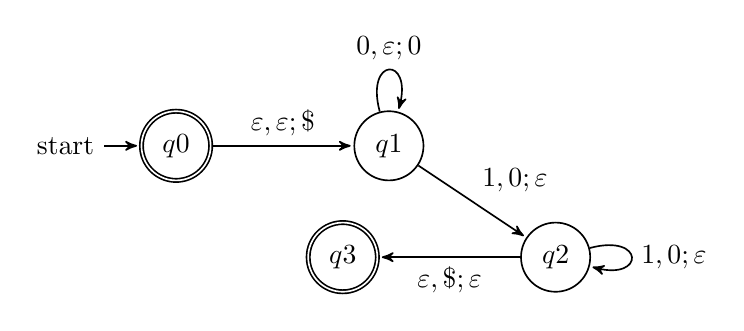
\begin{tikzpicture}[->,>=stealth',shorten >=1pt, auto, node distance=2cm, semithick]
    \tikzstyle{every state}=[text=black, fill=none]
    
    \node[initial,state,accepting] (q0)          {$q0$};
    \node[state]         (q1) [right of=q0, xshift=20pt] {$q1$};
    \node[state]         (q2) [below right of=q1, xshift=20pt] {$q2$};
    \node[state,accepting]         (q3) [left of=q2, xshift=-20pt] {$q3$};
    
    \path (q0) edge [bend left=0] node {$\varepsilon, \varepsilon; \$$} (q1)
        (q1) edge  [loop above] node {$0, \varepsilon; 0$} (q1)
        (q1) edge [bend left=0] node {$1, 0; \varepsilon$} (q2)
        (q2) edge  [loop right] node {$1, 0; \varepsilon$} (q2)
        (q2) edge  [bend left=0] node {$\varepsilon, \$; \varepsilon$} (q3)
    ;
\end{tikzpicture}

The PDA with state diagram above can be informally described as:
\begin{quote}
    Read symbols from the input. As each 0 is read, push it onto the stack. 
    As soon as 1s are seen, pop a 0 off the stack for each 1 read. 
    If the stack becomes empty and we are at the end of the input string, accept the input. 
    If the stack becomes empty and there are 1s left to read, 
    or if 1s are finished while the stack still contains 0s, or if any 0s
    appear in the string following 1s, 
    reject the input.
\end{quote}
    

Trace a computation of this PDA on the input string $01$.

\vfill
    
{\it Extra practice}: Trace the computations of this PDA on the input string $011$.

\vfill

\newpage
A PDA recognizing the set $\{ \hspace{1.5 in} \}$ can be informally described as:
\begin{quote}
    Read symbols from the input. As each 0 is read, push it onto the stack. 
    As soon as 1s are seen, pop a 0 off the stack for each 1 read. 
    If the stack becomes empty and there is exactly one 1 left to read, read that 1 and accept the input. 
    If the stack becomes empty and there are either zero or more than one 1s left to read, 
    or if the 1s are finished while the stack still contains 0s, or if any 0s appear in the input following 1s, 
    reject the input.
\end{quote}
Modify the state diagram below to get a PDA that implements this description:

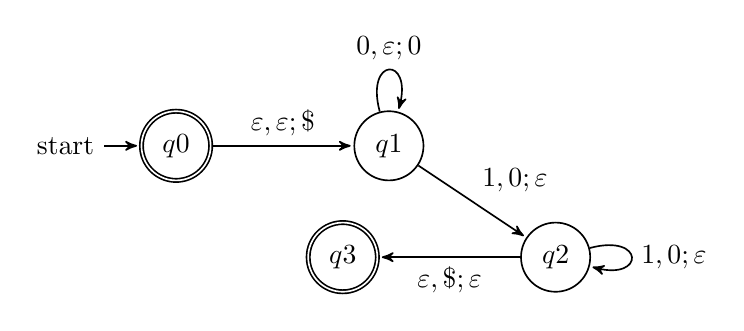
\begin{tikzpicture}[->,>=stealth',shorten >=1pt, auto, node distance=2cm, semithick]
    \tikzstyle{every state}=[text=black, fill=none]
    
    \node[initial,state,accepting] (q0)          {$q0$};
    \node[state]         (q1) [right of=q0, xshift=20pt] {$q1$};
    \node[state]         (q2) [below right of=q1, xshift=20pt] {$q2$};
    \node[state,accepting]         (q3) [left of=q2, xshift=-20pt] {$q3$};
    
    \path (q0) edge [bend left=0] node {$\varepsilon, \varepsilon; \$$} (q1)
        (q1) edge  [loop above] node {$0, \varepsilon; 0$} (q1)
        (q1) edge [bend left=0] node {$1, 0; \varepsilon$} (q2)
        (q2) edge  [loop right] node {$1, 0; \varepsilon$} (q2)
        (q2) edge  [bend left=0] node {$\varepsilon, \$; \varepsilon$} (q3)
    ;
\end{tikzpicture}
    
 

\end{document}